\documentclass[12pt,fleqn]{article}
\setlength{\parindent}{0pt}
\usepackage{graphicx}
\usepackage{listings}
\usepackage[latin5]{inputenc}
\setlength{\parskip}{8pt}
\setlength{\parsep}{0pt}
\setlength{\headsep}{0pt}
\setlength{\topskip}{0pt}
\setlength{\topmargin}{0pt}
\setlength{\topsep}{0pt}
\setlength{\partopsep}{0pt}
\setlength{\mathindent}{0cm}

\begin{document}
MIT OCW Cok Degiskenli Calculus - Ders 8

Iki degiskenli bir fonksiyonu grafiklemek (plot) icin 

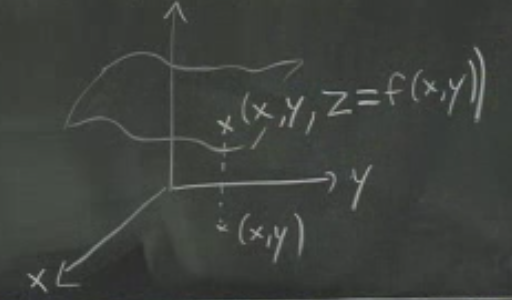
\includegraphics[height=4cm]{8_1.png}

$x,y$ degerlerine tekabul eden $f(x,y)$'yi, z ekseni uzerindeki yukseklik
olarak kabul ederiz, ve oraya bir nokta koyariz. Tum $x,y$'ler icin bu
yapilirsa bir yuzey ortaya cikar. Dikkat 3 boyutlu bir sekil gorulecektir,
fakat ici dolu degildir, fonksiyon sadece yuzeydedir. 

Ornek

\[ f(x,y) = -y \]

2 degiskenli de olsa illa her iki degisken fonksiyonda kullanilmali diye
bir sart yok. Bu formul bir duzlem tanimlar. 

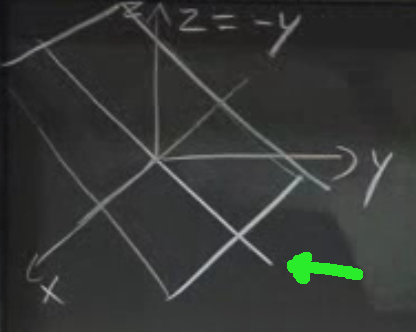
\includegraphics[height=4cm]{8_2.png}

Hoca cizmek icin once yesil okun gosterdigi cizgiden basladi, ki bu cizgi
$z=-y$, -1 egimi olan bir cizgi. $x$ tanimli olmadigina gore bu cizgi her
$x$ icin gecerli olmali, ve ustteki duzlem ortaya cikiyor. x-ekseni bu
duzlemin icinden geciyor. 

Ornek 

\[ f(x,y) = 1-x^2-y^2 \]

Grafigi anlamak icin $yz$ duzleminde neler oluyor onu anlamaya
ugrasalim. Sadece $yz$ duzlemine bakmak demek, $x=0$ kabul etmek demektir,
o zaman geri kalanlar 

\[ z = 1-y^2 \]

bir parabolu tanimlar. 

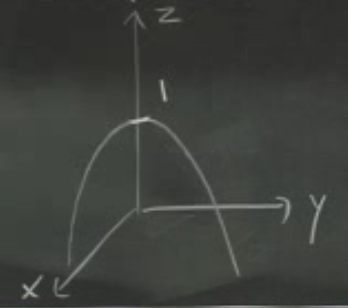
\includegraphics[height=4cm]{8_3.png}

Peki $xz$ duzleminde neler olur?

\[ z = 1- x^2 \]

yine asagi donuk bir parabol. 

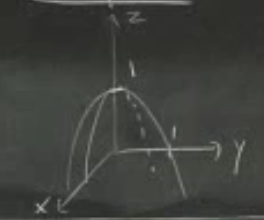
\includegraphics[height=4cm]{8_4.png}

$xy$ duzlemiyle nerede kesisim olur? $z=0$ ise, 

\[ 1-x^2-y^2 = 0 \]

\[ x^2 + y^2 = 1 \]

Bu birim yaricapi olan bir cemberdir (unit circle). 

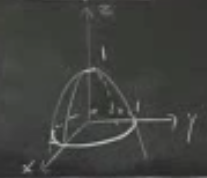
\includegraphics[height=4cm]{8_5.png}

Ilginc bir diger fonksiyon

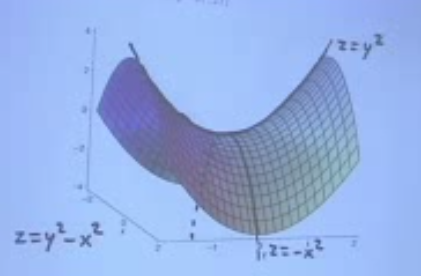
\includegraphics[height=4cm]{8_6.png}

Bir at egerine (saddle) benziyor, $yz$ duzleminden bakilinca yukari giden
bir parabol $z=y^2$, ama $xz$ duzleminde asagi donuk bir parabol, $z=-x^2$. 

Kontur Grafikleri (Contour Plot)

2 degiskenli fonksiyonlari cizmenin bir diger yolu onun konturlarini
cizmektir. Konturlar yeryuzunu resmetmek icin kullanilan haritalara
benzerler, 3 boyutlu sekillerin yassilastirilarak, sadece ustten
gorunuslerini gosteren grafikleme sekilleridirler. 

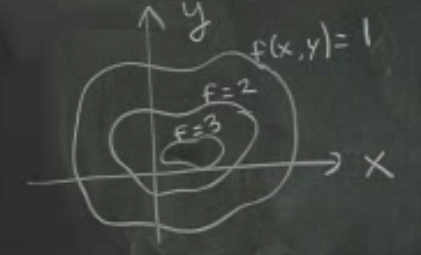
\includegraphics[height=4cm]{8_7.png}

Bir kontur grafigi uzerindeki cizgilerin her biri, bir yukseklige
(elevation) tekabul eder. Mesela $f(x,y)=1$ esitligi icin olan tum $x,y$
noktalari ustte en distaki kapali egridir, $f=2$, $f=3$, vs ayni sekilde. 3
boyutlu ``normal'' bir grafikte yukseklik olarak (3. boyut) temsil edilen
degerler yassilastirilarak onlarin ustten gorunusu resmedilir. Ayrica bir
$z$ ``sabitlenerek'' ona tekabul eden $x,y$ grafiklenir (bu sabit degerler
cogunlukla duzenli araliklarla olacak sekilde secilir, 1,2,3,4,vs gibi), 3
boyutlu bir resimde tum $z$ degerleri grafiklenir. Farkliliklar
bunlardir. Konturlar kullanarak 3 boyutlu bir fonksiyonu iki boyutta kismen
temsil edebilmis oluruz. 3 boyutlu fonksiyon ve $z=1$ anindaki bir kesit
ornegi alttadir. 

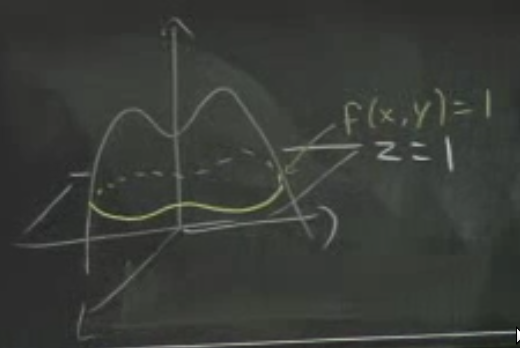
\includegraphics[height=4cm]{8_8.png}

Bu teknige ``seviye egrileri (level curve)'' ismi de verilir. $z=1$
seviyesinde kesit yapilinca o kesit uzerinde bir egri olusur, diger
seviyelerde de kesitler yapilabilir, vs. 

Bir topografik harita da aslinda bir kontur grafigidir. Mesela alttaki
harita ABD Jeolojik Olcumler (US Geological Survey) haritalarindan biri

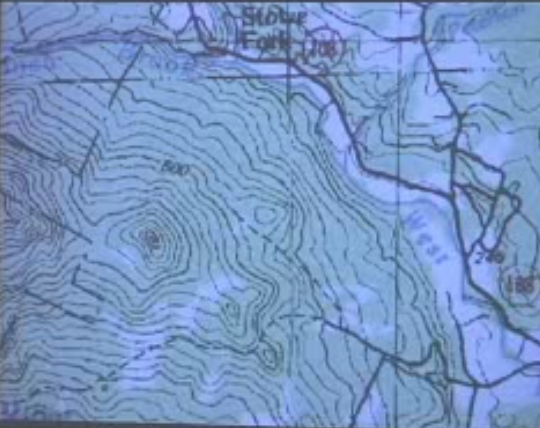
\includegraphics[height=4cm]{8_9.png}

Mesela 500 yazan bir cizgi var, bu yuksekligi gosteriyor. Eger o
yukseklikte kalmak istersek, hep o cizgi uzerinde yuruyebilirdik, ve hic
yukari ya da asagi gitmemis olurduk. Eger cizgiler arasinda gidip gelirsek,
o zaman yukseklik degisimi yapmis olurduk. 

Tabii kontur grafiklerinin illa bir cografi yuksekligi temsil etmesi
gerekmez. Mesela alttaki grafik ABD haritasinda herhangi kac derece
sicaklik oldugunu bolgesel olarak gosteriyor. 

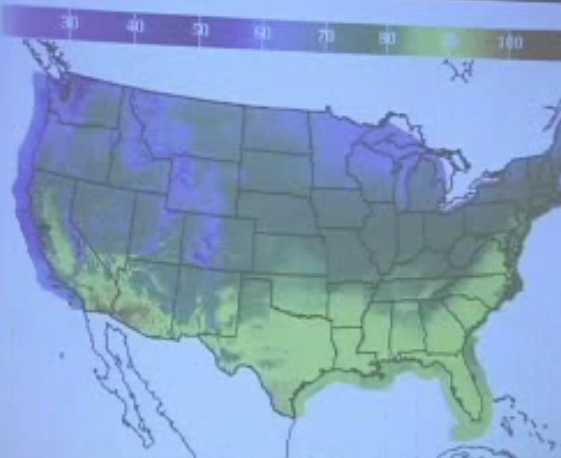
\includegraphics[height=4cm]{8_10.png}

Renkler belli sicakliklari temsil ediyorlar, ve renkler arasinda bazi
sinirlar var. Bu grafik te bir kontur grafigidir. 

Ornek

\[ f(x,y) = -y \]

Konturlar neye benzer? 

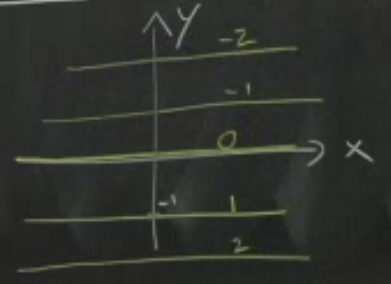
\includegraphics[height=4cm]{8_11.png}

Konturlar degisik yukseklikleri temsil ediyor, ve ustteki resim icin de bu
gecerli. Bu grafigin 3D hali icinde yesil ok olan en ustten 2. grafik. O
grafikte bir duz yokus var, iste ustteki cizgiler, bu yokustaki yukseklik
farkinda tekabul ediyorlar. 

Ornek

\[ f(x,y) = 1-x^2-y^2 \]

Bu fonksiyon sifir ise birim cember olur dedik, yani

\[ x^2+y^2=1 \]

Eger $f=1$ ise

\[ x^2+y^2=0 \]

Eger $f=-1$ ise

\[ x^2+y^2=2 \]

Eger $f=-2$ ise

\[ x^2+y^2=3 \]

Grafik soyle

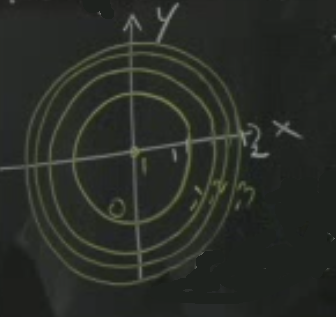
\includegraphics[height=4cm]{8_12.png}

Seviye egrilerinin disa dogru nasil daha s�kla�t���na dikkat cekmek
isterim. Bu demektir ki disa dogru gittikce yukseklik artisi daha dik hale
geliyor, cunku (yukari dogru) ayni birim mesafeyi almak icin gittikce daha
az mesafe katetmek gerekiyor. Orta kisim neredeyse dumduz. 

Ornek

At egrisi grafiginin konturlari

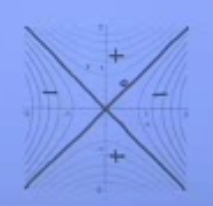
\includegraphics[height=4cm]{8_13.png}

Kontur grafikleri bize $x,y$ degisirken neler oldugunu soyler. Mesela
degerler azaliyor mu, cogaliyor mu? Bu tur bir sorunun cevabini kontur
grafigi hizli bir sekilde saglayabilir. 

Mesela su grafige bakalim

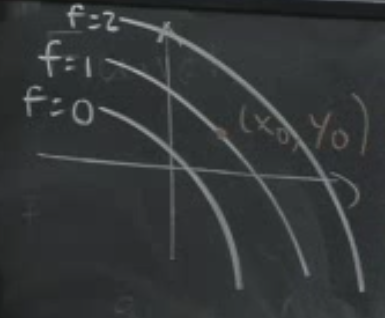
\includegraphics[height=4cm]{8_14.png}

Eger $x$ $\uparrow$, $f(x,y)$ $\uparrow$

Eger $x$ $\downarrow$, $f(x,y)$ $\downarrow$

Eger $y$ $\uparrow$, $f(x,y)$ $\uparrow$

Eger $y$ $\downarrow$, $f(x,y)$ $\downarrow$

Bu tur nicelik analiz kontur grafiklerinin cizgilerine bakarak hemen
yapilabilir. Ama belki de ben daha detayli bir analiz istiyorum, mesela
bir degiskeneki bir degisimin $f(x,y)$'daki degisimi ne kadar etkiledigini
detayli sekilde gormek istiyorum.

Degisim oranlarinin hesabi turevlerle yapilir. 

Kismi Turevler (Partial Derivatives)

Tek degiskenli fonksiyonlar, mesela $f(x)$ gibi, o zaman $f(x)$'in turevi
bir limit olarak tanimlidir

\[ f'(x) = \frac{df}{dx}  = 
\lim_{\Delta x \to 0} \frac{f(x+\Delta x) - f(x)}{\Delta x}
\]

Grafiksel olarak

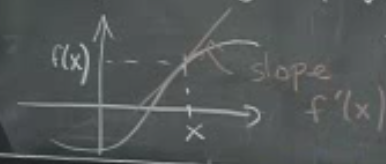
\includegraphics[height=3cm]{8_15.png}

$x$ noktasindaki egim (slope) $f'(x)$'e esittir. 











\end{document}
